%\setchapterimage{fig_00.jpg}
\chapter*{Application \arabic{cptApplication} \\ 
Stabilité des systèmes -- \ifprof Corrigé \else Sujet \fi}
\addcontentsline{toc}{section}{Application \arabic{cptApplication} : Stabilité des systèmes  -- \ifprof Corrigé \else Sujet \fi}

\iflivret \stepcounter{cptApplication} \else
\ifprof  \stepcounter{cptApplication} \else \fi
\fi

\setcounter{question}{0}
%\marginnote{Concours Centrale -- MP 2019}
\marginnote{
\UPSTIcompetence[2]{C1-01}
\UPSTIcompetence[2]{C2-03}
}


%\subsection*{Exercice 1 -- Réponse impulsionnelle (entrée Dirac)}

On considère le schéma-blocs ci-contre et la réponse indicielle pour $K_C=1$.
\begin{marginfigure}
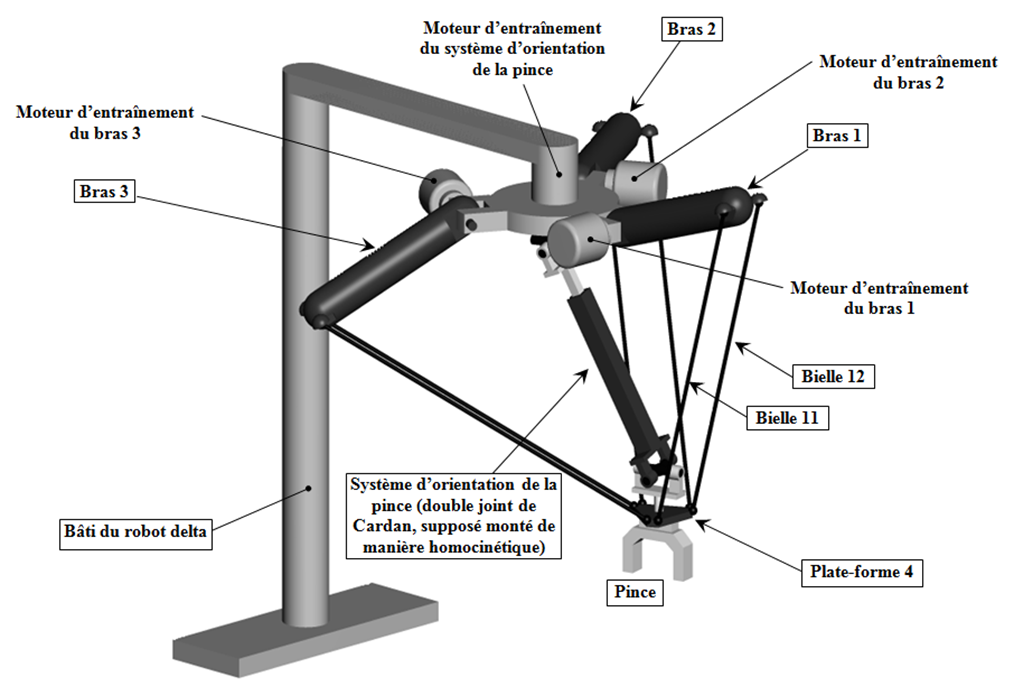
\includegraphics[width=\linewidth]{fig_01}
\end{marginfigure}


\question{Justifier l'allure du diagramme du diagramme de Bode donné ci-dessous pour $K_C=1$.}

\begin{figure}[!h]
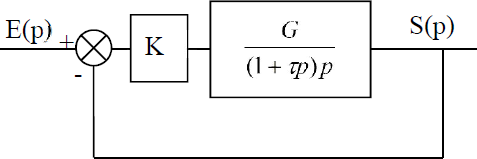
\includegraphics[width=.8\linewidth]{fig_02}
\end{figure}

\question{Donner graphiquement les marges de phase et de gain pour $K_C=1$.}
\ifprof
\begin{center}
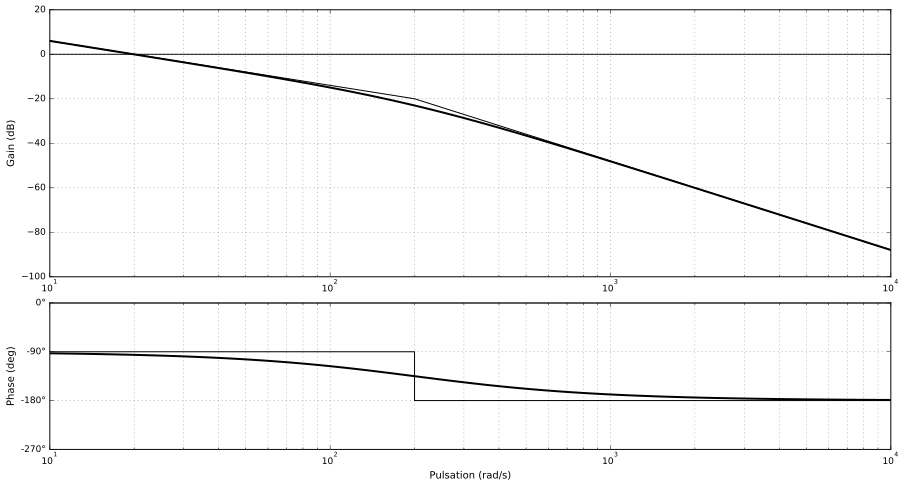
\includegraphics[width=\linewidth]{cor_01}
\end{center}

\else
\fi


\question{Donner analytiquement les marges de phase et de gain pour $K_C=1$ (méthode).}
\ifprof
\begin{corrige}
\textbf{Calcul de la marge de gain}
\begin{itemize}
\item On détermine $\omega_{180}$ tel que $\arg\left(\text{FTBO}(j\omega_{180})\right)=-180\degres$. 

$\arg\left(\text{FTBO}(j\omega)\right) $ $= -\arg\left( j\omega\right)-\arg\left( 1+ 10 j\omega\right)-\arg\left(1+0,5j\omega \right) $ $= - 90 - \arctan \left( 10 \omega \right) - \arctan \left( 0,5 \omega \right)$.

$\arg\left(\text{FTBO}(j\omega_{180})\right)=-180\degres$ 
$\Leftrightarrow - 90 - \arctan \left( 10 \omega \right) - \arctan \left( 0,5 \omega \right) = -180$

\begin{lstlisting}
import math as m
from pylab import *
from scipy.optimize import bisect 

def f(x):                                       
    res = m.pi/2 - m.atan(10*x) - m.atan(0.5*x)
    return res

zero1 = bisect(f, .1, 10)
\end{lstlisting}
On a $\omega=\SI{0,447}{rad.s^{-1}}$.
%$\Leftrightarrow - \arctan \left( 10 \omega \right) - \arctan \left( 0,5 \omega \right) = -90$
\end{itemize}

\end{corrige}
\else
\fi

\question{Le cahier des charges impose des marges de gain et de phase minimales de \SI{12}{dB} et 40\degres. Déterminer
la plus grande valeur de $K_C$ permettant de vérifier ce cahier des charges}





\ifprof
\else
\begin{figure}[h!]
\centering

%\begin{minipage}{.45\textwidth}
%\centering
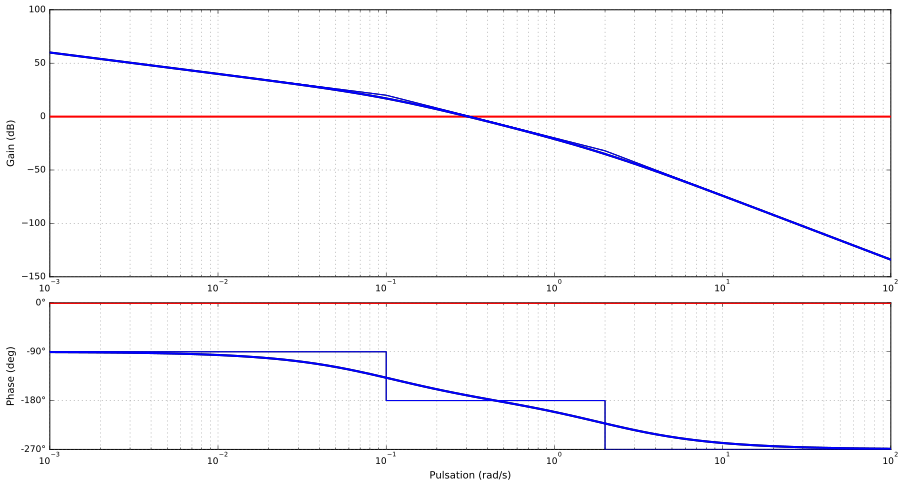
\includegraphics[width=\linewidth]{fig_03}
%\end{minipage}%
%\begin{minipage}{.45\textwidth}
%\centering
%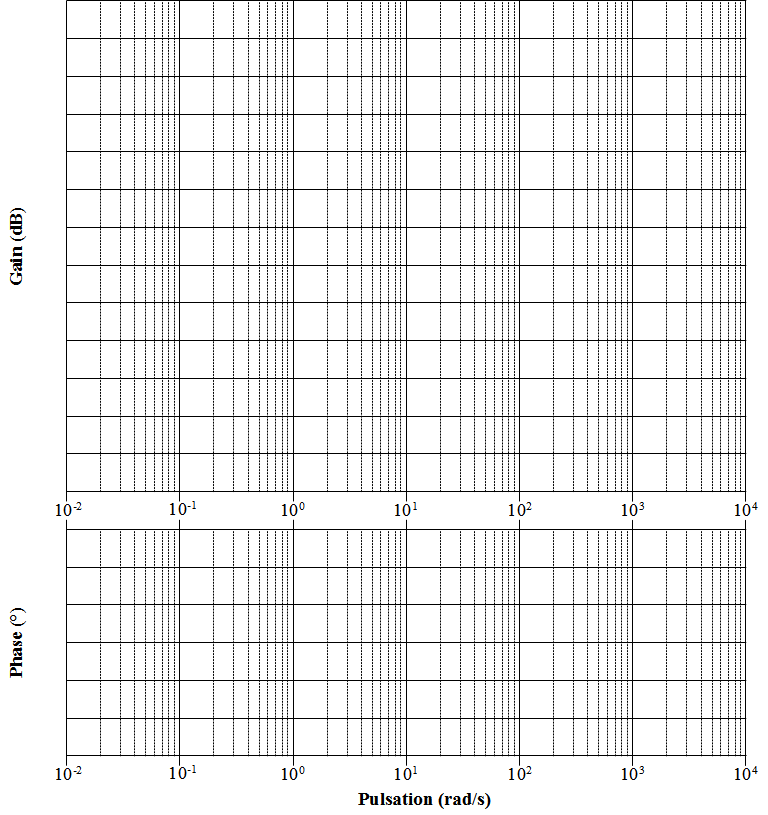
\includegraphics[width=\linewidth]{img_04}
%\end{minipage}
\end{figure}
\fi


\ifprof
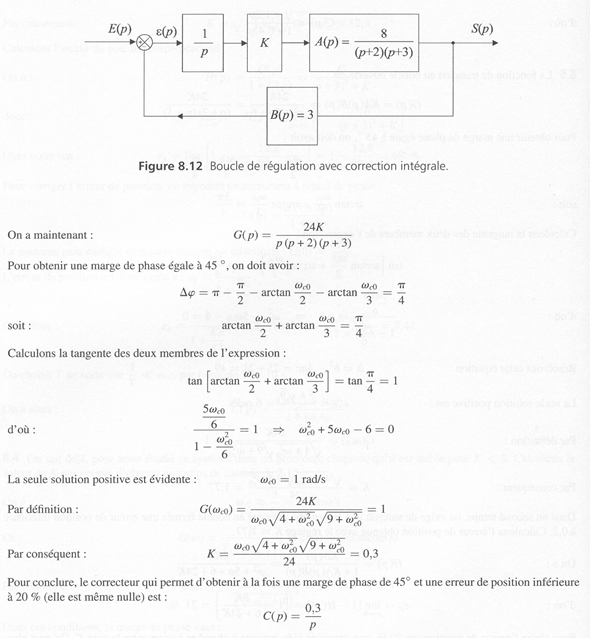
\includegraphics[width=\linewidth]{cor_02}
\end{center}
\else
\fi


%\ifprof
%\else
%\noindent\begin{minipage}[c]{.4\linewidth}
%\begin{center}
%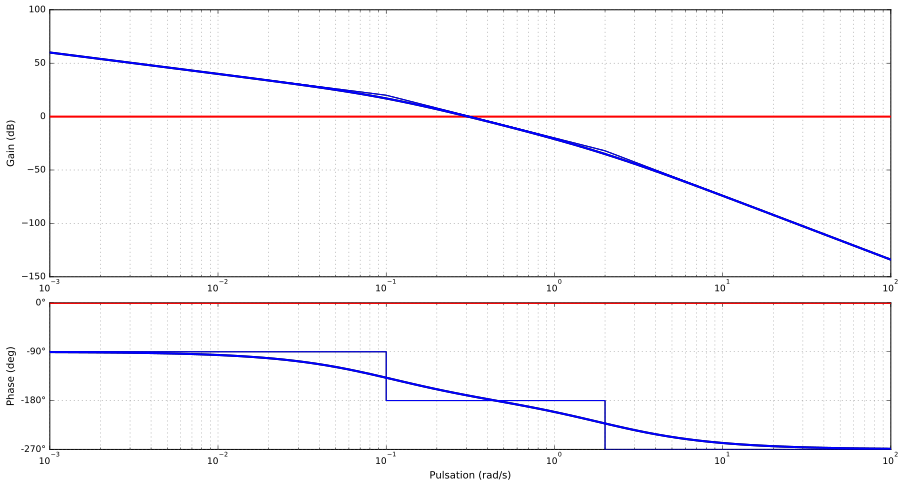
\includegraphics[width=\linewidth]{fig_03}
%\end{center}
%\end{minipage}\hfill
%\begin{minipage}[c]{.46\linewidth}
%\begin{center}
%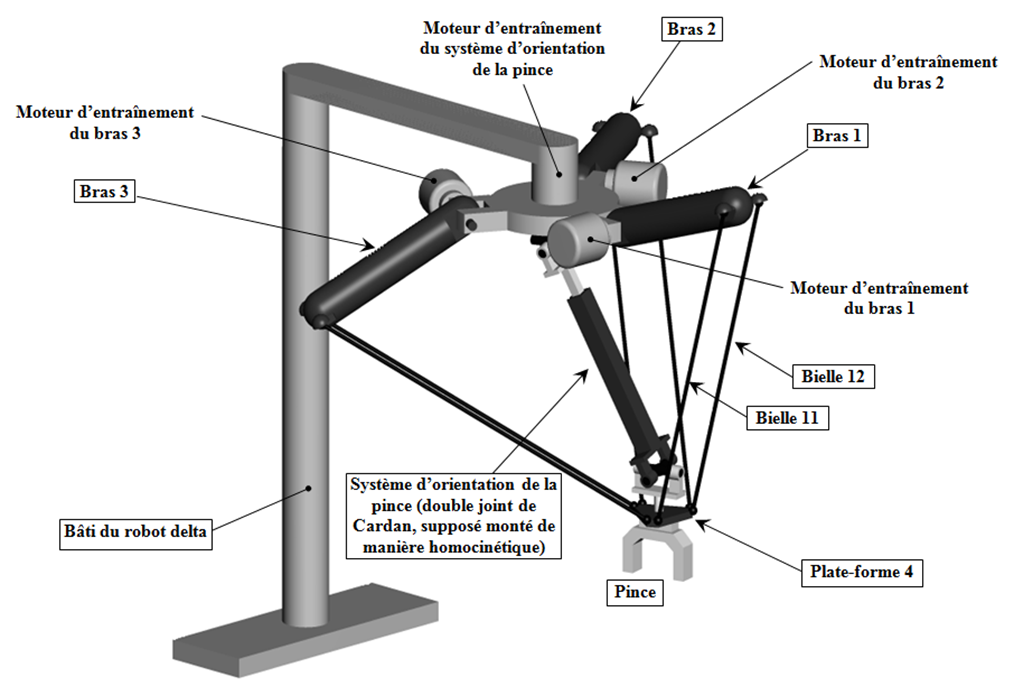
\includegraphics[width=.9\linewidth]{fig_01}
%\end{center}
%\end{minipage}

%
%\begin{center}
%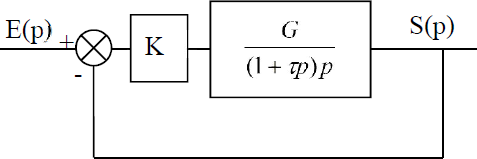
\includegraphics[width=\linewidth]{fig_02}
%\end{center}
%
%\begin{center}
%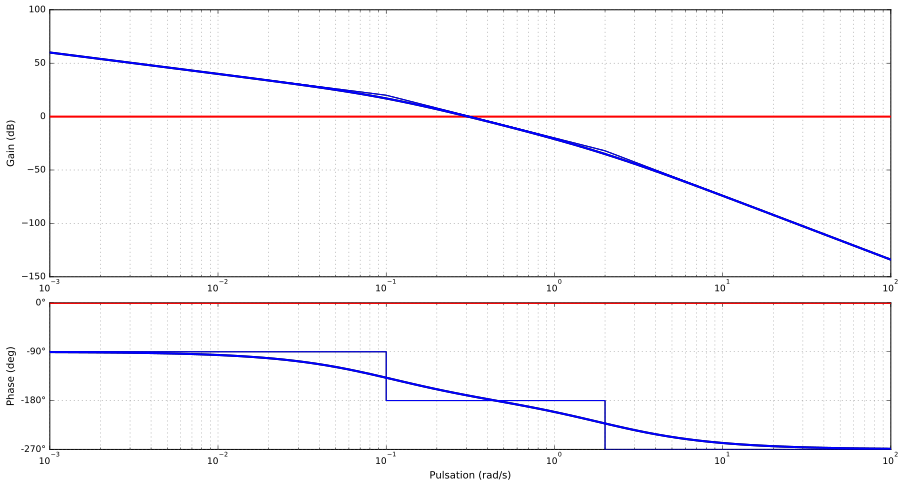
\includegraphics[width=\linewidth]{fig_03}
%\end{center}
%
%\begin{center}
%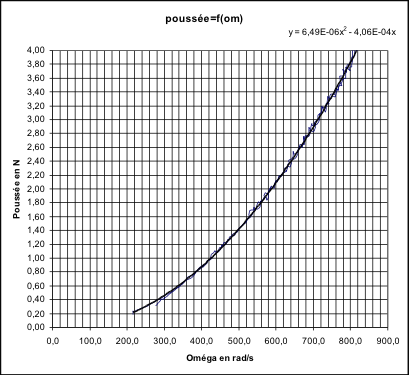
\includegraphics[width=.8\linewidth]{fig_04}
%\end{center}


%
%\end{document}
%
%\subsection*{Exercice 3 -- Applications du critère du Revers}
%
%\subparagraph*{}\textit{On donne ci-dessous les lieux de transferts de plusieurs FTBO. Déterminer, à l'aide du critère du Revers si les systèmes sont stables en BF.}
%\subparagraph*{}\textit{Pour les systèmes stables déterminer les marges de gain et de phase.}
%
%\end{multicols}
%
%\begin{center}
%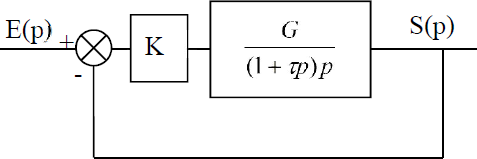
\includegraphics[width=\linewidth]{fig_02}
%\end{center}
%
%\begin{center}
%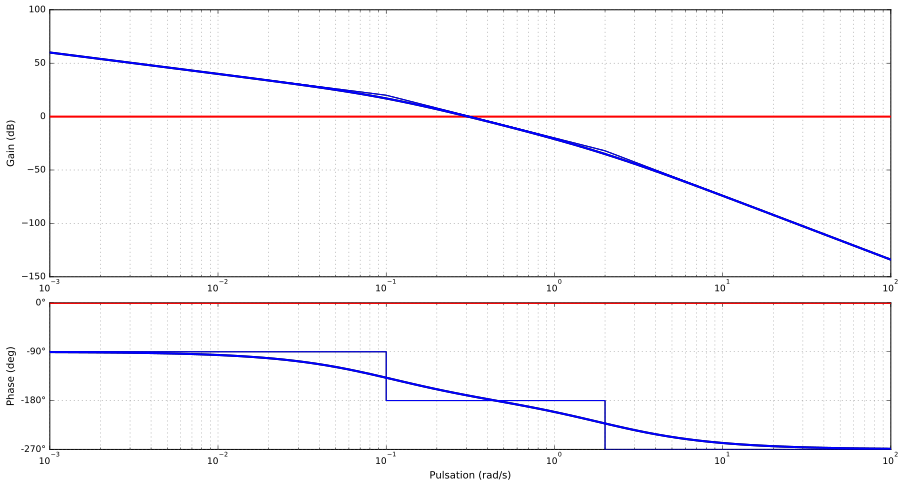
\includegraphics[width=\linewidth]{fig_03}
%\end{center}
%
%\begin{center}
%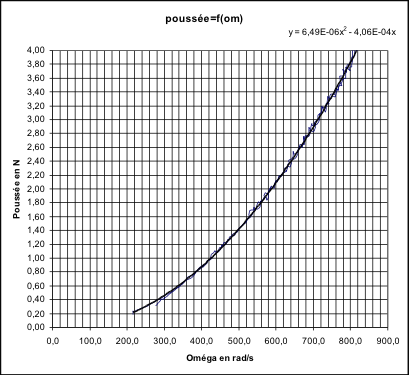
\includegraphics[width=.8\linewidth]{fig_04}
%\end{center}



